\documentclass{dcbl/challenge}

\setdoctitle{K-Map}
\setdocauthor{Stephan Bökelmann}
\setdocemail{sboekelmann@ep1.rub.de}
\setdocinstitute{AG Physik der Hadronen und Kerne}
\usepackage{graphicx}
\usepackage{caption}



\begin{document}
The combination of basic logic operators is a powerful tool in computing.
Any statement that can be formulated in terms of propositional logic, can be implemented using the basic logic operators. 
In order to find a way to implement a statement, a commonly used method is the generation of a \textit{truth table}.
These truth tabels can also be transformed in what is called a \textit{K-Map}.
Expressed in this particular form, statements for a logic output can be written down in a straightforward way. 
By finding rectangular cells of ones or zeros in a K-Map, it is possible to find a statement for a logic output.
\section*{Exercises}
\begin{aufgabe}
    Write down the truth-table for an OR-gate that maps the inputs $A$ and $B$ to the output $Q$. 
    Consecutively, write down a $2x2$ grid, with the columns representing $A=0$ and $A=1$ as well as the rows representing $B=0$ and $B=1$.
    Take a different color of pen and circle rectangular cells of ones in this K-Map. 
    You will end up with two rectangular cells, both representing the output $Q=1$.
    The output of this logic function can now be expressed as $Q$ is true if either the prerequisites for circle 1 or circle 2 are fullfilled. 
    Take a look at which prerequisite is stable for a given rectangular cell and which one doesn't have an influence. 
    All prerequisites that are constant for a given rectangular cell have to be joined by an AND-gate.
    This is how you can come up with an expression for rectangular cell. 
    Joining n individual cells is done by using an OR-gate.
    You should now see, that looking at the K-Map and the rectangular cells, the circled cells reproduce the statement of $Q = A or B$
\end{aufgabe}
\begin{aufgabe}
    Take a look at table \ref{fig:ABC}. 
    Find all rectangular cells.
    You will now also see, that there is no way of expressing rectangular cells with an amount of cells, that is not divisible by $2^n$.
    Write down the boolean-statment that is represented by the given K-Map.\\
    \begin{figure}
        \centering
        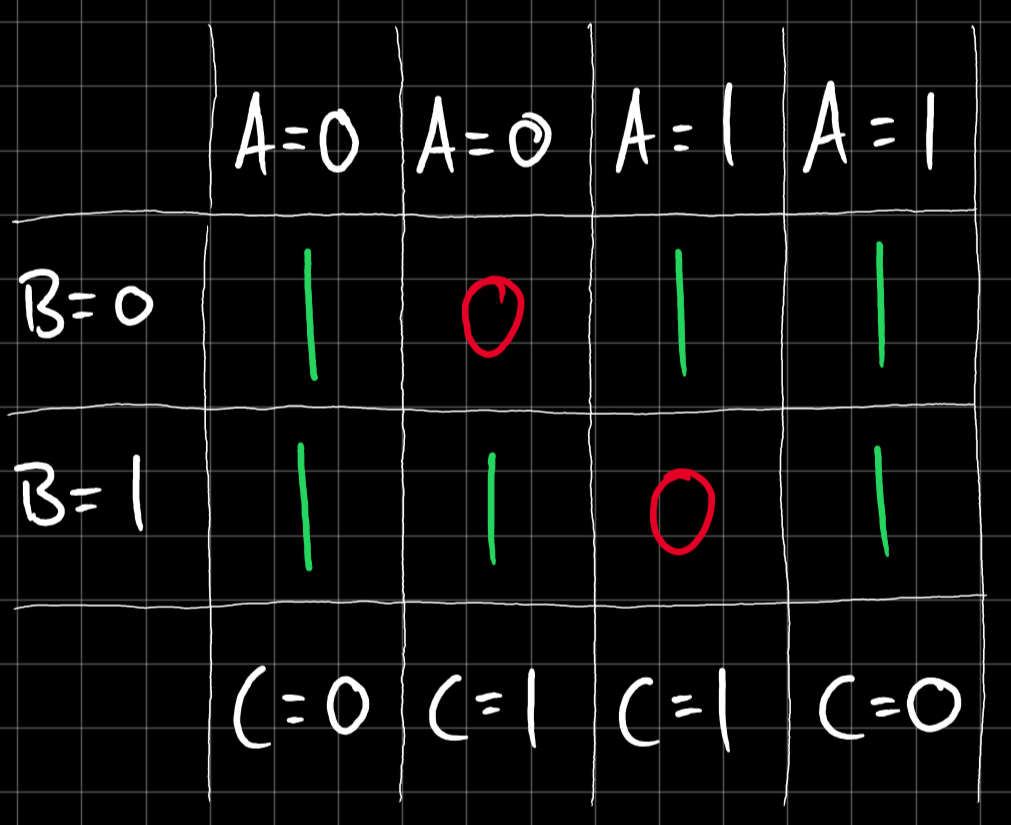
\includegraphics[width=.4\linewidth]{ABC.png}
        \captionof{figure}{Three Input K-Map}
        \label{fig:ABC} 
    \end{figure}
\end{aufgabe}
\begin{aufgabe}
    A K-Map usually only represents the statement of a single output. 
    When confronted with multiple outputs as seen in table \ref{fig:adder}, one will have to create a K-Map for each output.
    Thus, each output is represented by an individual equation, resulting in an individual circuit. 
    Write down the K-Maps for the truth table in table \ref{fig:adder}.
    \begin{figure}
        \centering
        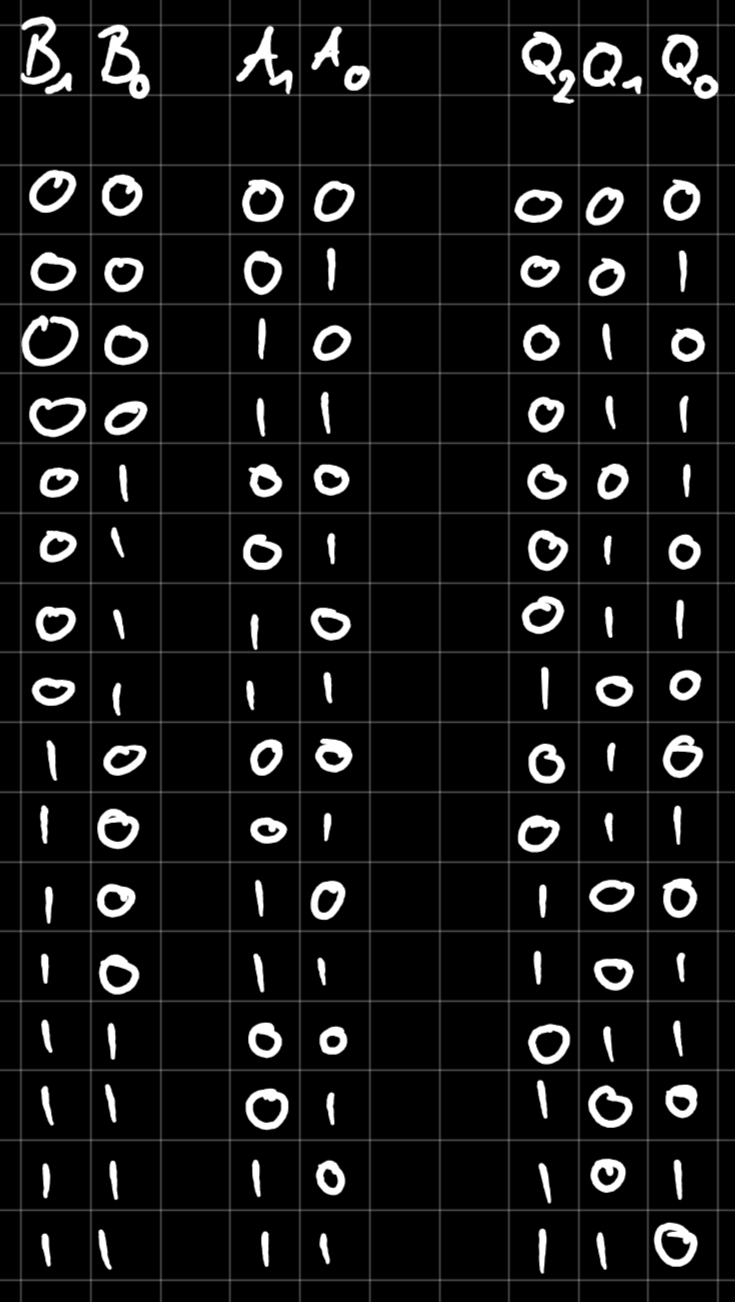
\includegraphics[width=.6\linewidth]{ADDER.png}
        \captionof{figure}{Truth Table with Multiple Outputs}
        \label{fig:adder} 
    \end{figure}
\end{aufgabe}


\section*{Annotations}
\begin{enumerate}
    \item Worksheet \textit{Naive Logic Gates}: \url{https://github.com/bjoekeldude/4e30ea01-26e6-4037-9a12-7ccc98bc70ee}
    \item \url{https://en.wikipedia.org/wiki/Karnaugh_map}
    \item Introduction to K-Maps on YouTube: \url{https://www.youtube.com/watch?v=RO5alU6PpSU}
\end{enumerate}

\end{document}
